\section{Resolución Problema 4}
\subsection{Problema:}
Dado un numero decimal entero positivo o negativo regresar su equivalente en binario.


\subsection{\textbf{Descripción del problema:}}
Dado un numero decimal entero positivo o negativo regresar su equivalente en binario.

\subsection{\textbf{Definición de solución:}}
El informe analiza el proceso de conversión de un número decimal entero positivo o negativo a su representación binaria. Se resalta la relevancia de comprender, en el ámbito de las matemáticas discretas, cómo un número experimenta este cambio de representación.
\newline


\item[{\ieeeguilsinglright}] {\it A. DECIMALES POSITIVOS }
   
La conversión de números decimales enteros positivos a binarios, esta basada en divisiones sucesivas por 2. 
\newline

\begin{figure}[h!]
    \centering
    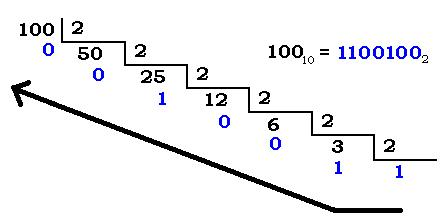
\includegraphics[width = 6 cm]{./latex-imágenes/conversion.jpg}
    \caption{Proceso de conversión de 100 utilizando la técnica de sucesivas divisiones por dos}
    \vspace*{-5pt}
    \label{fig:dos}
\end{figure}


\item[{\ieeeguilsinglright}] {\it B. DECIMALES NEGATIVOS }

Por n el caso de números negativos, el proceso se complica y se introduce el concepto de complemento 1 y 2.

\begin{itemize}
    \item Complemento a 1:
\end{itemize}
En el contexto del "complemento a 1" de un número binario, nos referimos a la secuencia de bits que se obtiene al invertir (cambiar de 0 a 1 y de 1 a 0) todos los bits del número original. 
\newline

Por ejemplo, si tenemos el número binario 01010101, al aplicar el complemento a 1 obtendríamos 10101010, ya que hemos invertido cada bit. El complemento a 1 se utiliza principalmente para representar la magnitud negativa de un número binario y es una parte fundamental en el cálculo del complemento a 2."
\newline

\begin{itemize}
    \item Complemento a 2:
\end{itemize}
El proceso de obtener el complemento a 2 de un número binario es un paso esencial en la representación de números negativos en sistemas binarios. Este método se basa en la utilización del complemento a 1 y la adición de 1 al resultado
\newline

\begin{figure}
\centerline{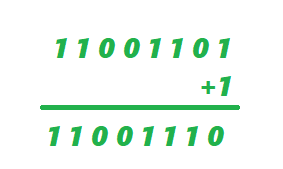
\includegraphics[width=18.5pc]{./latex-imágenes/complementoADos}}
\caption{Proceso de conversión de 100 utilizando la técnica de sucesivas divisiones por dos}
\vspace*{-5pt}
\label{fig:dos}
\end{figure}

\subsection{\textbf{Diseño de la solución:}}

\begin{itemize}
    \item Solicitar al usuario que ingrese un número decimal entero positivo o negativo en el rango de 64 bits, específicamente entre -1024 y 1024.
    \item Lee la entrada del usuario y almacena el valor en la variable numeroD.
    \item Verifica si numeroDecimal está en el rango permitido. Si es positivo, realiza la conversión a binario. Si es negativo, calcula los complementos a uno y a dos.
    \item Si el número está fuera del rango, lanza un mensaje de error.
    \newline 
    
    \newline NÚMEROS ENTEROS POSITIVOS:
    \item Utiliza un bucle para realizar sucesivas divisiones por 2, registrando los residuos como bits en la representación binaria.

    
    \begin{figure}
        \centerline{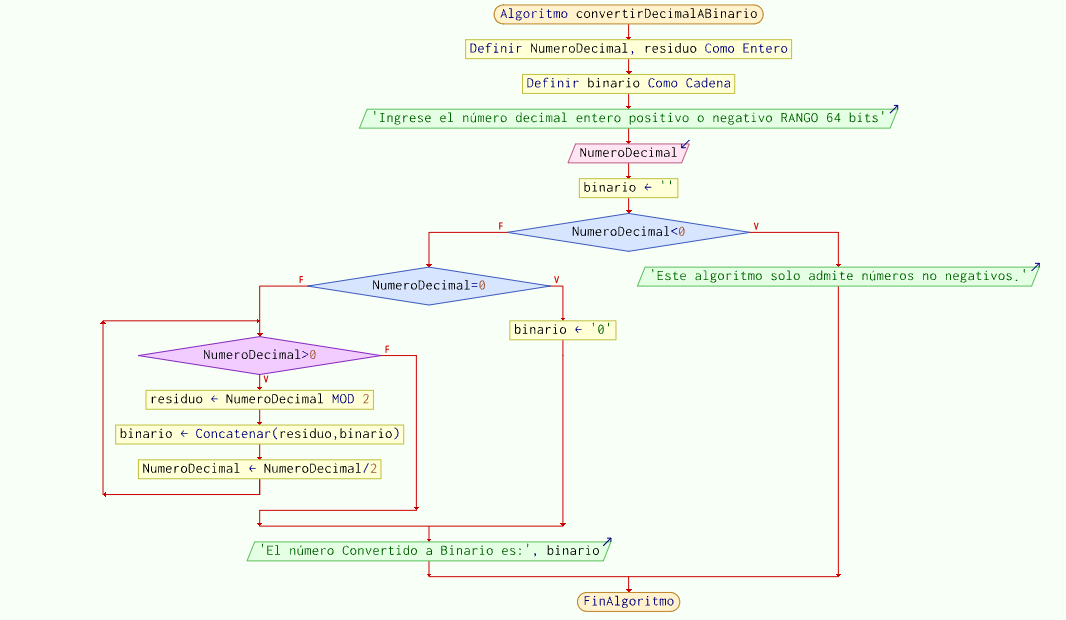
\includegraphics[width=18.5pc]{./latex-imágenes/diagramaDecimalABinarioPositivo.png}}
        \caption{Diagrama de flujo en caso de ser números Positivos}
        \vspace*{-5pt}
        \label{fig:dos}
        \end{figure}


    \newline NÚMEROS ENTEROS NEGATIVOS:
    \item Para complemento a Uno, utiliza la representación binaria obtenida anteriormente.
    \item Determina la longitud de bits necesarios para representar el número según su rango.
    \item Añade ceros a la izquierda para alcanzar la longitud necesaria e invierte cada bit para obtener el complemento a uno.
    \newline 
    
    \item Para el complemento a dos utiliza la representación del complemento a uno.
    \item Agrega 1 al dato de número valor resultado para obtener la representación del complemento a dos.
    \item Utiliza la clase BigInteger para manejar números grandes, ya que la representación de 65 bits podría exceder la capacidad de un tipo de datos primitivo.
    \item Imprime el resultado de la conversión a binario o los complementos a uno y a dos, según sea el caso.
    \end{itemize}

        \begin{figure}
            \centerline{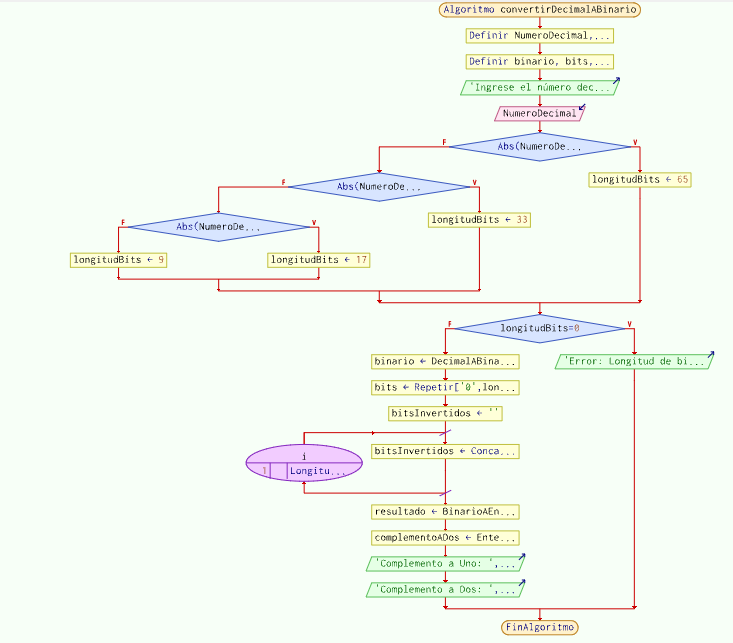
\includegraphics[width=18.5pc]{./latex-imágenes/diagramaDecimalABinarioNegativo.png}}
            \caption{Diagrama de Flujo en  caso de ser números negtivos }
            \vspace*{-5pt}
            \label{fig:dos}
            \end{figure}
            
            


\subsection{\textbf{Desarrollo de la solución:}}

El algoritmo de solución para la conversión: comienza importando librerías específicamente "Scanner" para capturar todo lo que ingrese el usuario y "BigInteger".

\newline

\begin{javaCode}
import java.math.BigInteger;
import java.util.Scanner;
\end{javaCode}

Se validan los datos: el número debe ser solo entero ya sea positivo o negativo entre el rango de 64 bits, dependiendo su valor va a imprimirlo de acuerdo al número ingresado.
\newline

\begin{javaCode}
   public static void main(String[] args) {
        Scanner decimal = new Scanner(System.in);

        
        // Solicitud del número decimal
        System.out.println("Ingrese el número decimal entero positivo o negativo RANGO 64 bits [-1024, 1024]: ");
        String numeroD = decimal.nextLine();

        // Convierte la variable a un número de tipo long 
        numeroDecimal = Long.parseLong(numeroD);

        // Valida el rango solicitado
        if (numeroDecimal >= -1024 && numeroDecimal <= 1024) {
            if (numeroDecimal >= 0) {
                // Impresión del número convertido en caso de ser positivo 
                System.out.println("El número convertido a binario es: " + decimalABinario());
            } else {
                //Impresión del número en caso de ser negativo 
                System.out.println("Complemento a 1: " + complementoAUno());
                System.out.println("Complemento a 2: " + complementoADos());
            }
    
}
\end{javaCode}

En caso contrario que el usuario haya tecleado un número diferente al solicitado , donde si se encuentra fuera del rango o sea otro tipo de valor va a arrojar un mensaje de "Error". 
\newline

\begin{javaCode}
    //Excepción en caso de no encontrase en el rango solicitado
    } else {
         System.out.println("Error: Formato no válido" );
    }
// Cerrar el scaneo 
decimal.close(); 
\end{javaCode}

En el método decimalABinario se crea una variable llamada "binario” tipo cadena, toma el valor de decimal y lo convierte en el valor absoluto, automáticamente si el número ingresado es 0 lo retornara.
\newline

\begin{javaCode}
    public static String decimalABinario() {
        String binario = "";
        // Convetir decimal a valor absoluto 
        long numero = Math.abs(numeroDecimal);

        if (numero == 0) {
            return "0";
        }
\end{javaCode}


Se crea un bucle para números distintos de 0, considerando su valor absoluto y permitiendo manejar números negativos y positivos. En el bucle, se divide el número por 2, concatenando su residuo de derecha a izquierda y actualizando su valor.
\newline

\begin{javaCode}
     // Bucle para convertir a número decimal
        while (numero != 0) {
            long residuo = numero % 2;
            binario = residuo + binario;
            numero = numero / 2;
        }
        return binario;
    }
\end{javaCode}

De acuerdo al número ingresado, se realiza una comparación de su rango con una estructura condicional. Sin embargo, debido a la necesidad de realizar una suma para calcular el complemento a dos, se sumara 1 bit.
\newline

\begin{javaCode}

    public static String complementoAUno() {
        // Obtener la representación binaria del número absoluto
        String binario = decimalABinario();

        // Determinar la longitud de bits necesarios
        int longitudBits;
        if (numeroDecimal >= -128 && numeroDecimal <= 128) {
            longitudBits = 9;
        } else if ((numeroDecimal >= 129 && numeroDecimal <= 256) || (numeroDecimal >= -256 && numeroDecimal <= -129)) {
            longitudBits = 17;
        } else if ((numeroDecimal >= 257 && numeroDecimal <= 512) || (numeroDecimal >= -512 && numeroDecimal <= -257)) {
            longitudBits = 33;
        } else if ((numeroDecimal >= 513 && numeroDecimal <= 1024) || (numeroDecimal >= -1024 && numeroDecimal <= -513)) {
            longitudBits = 65;
        } else {
            return "Error";
        }
\end{javaCode}

Se ajusta la longitud de la cadena con ceros, se invierte para construir el complemento utilizando StringBuilder y se devuelve como una cadena.
\newline

\begin{javaCode}
   // Añadir ceros a la izquierda según la longitud necesaria
        String bits = "0".repeat(Math.max(0, longitudBits - binario.length())) + binario;

        // Añadir ceros a la izquierda según la longitud necesaria
        String bits = "0".repeat(Math.max(0, longitudBits - binario.length())) + binario;

        // Invertir cada bit guardandolo en complemento 
         StringBuilder complemento = new StringBuilder();
        for (int i = 0; i < bits.length(); i++) {
            char bit = bits.charAt(i);
            complemento.append((bit == '0') ? '1' : '0');
        }
        return complemento.toString();
    }
\end{javaCode}

Por último calcula el complemento a dos de un número binario representado como cadena. Obtiene la representación binaria del complemento a uno, convierte a BigInteger (para 65 bits), suma 1 y devuelve la cadena del resultado. 

\begin{javaCode}
       public static String complementoADos() {
        // Obtener la representación del complemento a uno
        String binario = complementoAUno();

        // Agregar 1 al resultado para obtener la representación de complemento a 2
        //Declarar el resultado en BigInterger para numeros de 65 bits
        BigInteger resultado = new BigInteger(binario, 2).add(BigInteger.ONE);
        return resultado.toString(2);
    }
\end{javaCode}


\subsection{\textbf{Depuración y pruebas:}}

\begin{itemize}
    \item DECIMAL POSITIVO  
    

\begin{center}
    \begin{tabular}{|c|c|c|c|}
    \hline
    \textbf{Número Decimal} & \textbf{Número Binario} \\
    \hline
    7 & 111 \\
    \hline
    10 & 1010 \\
    \hline
    0  & 0  \\
    \hline
    \end{tabular}
\end{center}

  \item DECIMAL NEGATIVO  
\begin{center}
    \newline
    \begin{tabular}{|c|c|c|c|}
    \hline
    \textbf{Decimal} & \textbf{comp. a 1} & \textbf{comp. a 2} \\
    \hline
    -4 & 111111011 & 111111100 \\
    \hline
    -124 & 110000011 & 110000100\\
    \hline
    \end{tabular}
\end{center}
\end{itemize}